\section{Variable Metric Bundle Method}
\label{sec_variable_metric}

\textcolor{red}{can I call this variable metric method or does this imply variable metric updates and not solving the bundle subproblem?}
%\textcolor{blue}{introduction}

A way to extend the proximal bundle method is to use an arbitrary metric \(\frac{1}{2}\Langle d,W_kd \Rangle\) with a symmetric and positive definite matrix \(W_k\) instead of the Euclidean metric for the stabilization term \(\frac{1}{2t_k}\|d\|^2\). Methods doing so are called \emph{variable metric bundle methods}.
This section combines the method of Hare et al. presented in section \ref{sec_nonconv_inex} with the second order model function used by Noll in \cite{Noll2013} to a metric bundle method suitable for nonconvex functions with noise.

The section starts by explaining the ideas from \cite{Noll2013} used to extend the method presented above. It then gives an explicit strategy how to update the metric during the steps of the algorithm and concludes with a convergence proof for the developed method.

Throughout this section we still consider the optimization problem (\ref{opt_prob_nonconv_inex}). We also keep the names and definitions of the objects used in section \ref{sec_nonconv_inex}.

\subsection{The Main Ingredients to the Method}
%\textcolor{blue}{explanation}

As already mentioned in section \ref{sec_conv_ex} the stabilization term can be interpreted in many different ways. In the context of this section we can understand it as a pretty rough approximation of the curvature of the objective function.
Of course bundle methods are designed to work with non differentiable objectives so it cannot be expected that the function provides any kind of curvature. However, if it does, incorporating it into the method could speed up convergence.

\subsubsection{Variable Metric Bundle Methods}

Variable metric bundle methods use an approach that can be motivated by the thoughts stated above.
Instead of using the Euclidean norm for the stabilization term \(\frac{1}{2}\|d\|^2 \) the metric is derived from a symmetric and positive definite matrix \(W_k\). As the name of the method suggests, this matrix can vary over the iterations of the algorithm. The subproblem in the \(k\)'th iteration therefore reads 

\begin{equation*}
	\min_{\hat{x}^k+d \in \R^n} M_k(\hat{x}^k+d)+\mathtt{i}_{X}(\hat{x}^k+d)+\frac{1}{2}\Langle d,W_kd \Rangle.
\end{equation*}

As explained in \cite{Lemarechal1994} like (\ref{sub_prob_fin}) this is a Moreau-Yosida regularization of the objective function (on the constraint set), so this subproblem is still strictly convex and has a unique solution. It is however harder to solve especially if the matrices \(W_k\) are no diagonal matrices \cite{Luksan1999}.
In the unconstrained case or for a very simple constraint set the subproblem can be solved by calculating a quasi Newton step. Such a method is presented by Lemar\'{e}chal and Sagastiz\'{a}bal in \cite{Lemarechal1997} for convex functions. Luk\v{s}an and {Vl\v{c}ek} use an algorithm in those lines in \cite{Vlcek2001} which is adapted to a limited memory setting by Haarala et al. in \cite{Haarala2007}.

A challenging question is how to update the matrices \(W_k\). It is important that the updating strategy preserves positive definiteness of the matrices and that the matrices stay bounded. The updates that are used most often are the symmetric rank 1 formula (SR1 update) and the BFGS (Broyden-Fletcher-Goldfarb-Shanno) update. These updates make it possible to assure the required conditions with only little extra effort even in the nonconvex case. Concrete instances of the updates are given in \cite{Vlcek2001} and \cite{Lemarechal1994}.

%stabilization term mimics curvature \(\to\) more sophisticated in variable metric bundle methods \(\to\) explain those; examples \(\to\) Noll also kind of variable metric bundle method 

\subsubsection{Noll's Second Order Model}

In \cite{Noll2012} Noll et al. present a proximal bundle method for nonconvex objective functions. An important ingredient to the method is that not the objective function itself is approximated in the subproblem but a quadratic model of it:

\begin{equation}
	\Phi(x,\hat{x}) = \phi(x,\hat{x})+\frac{1}{2}\langle x-\hat{x},Q(\hat{x})(x-\hat{x})\rangle
\end{equation}

The first order model \(\phi(\cdot,\hat{x})\) is convex and possibly nonsmooth. The second order part \(\frac{1}{2}\langle \cdot-\hat{x},Q(\hat{x})(\cdot-\hat{x})\rangle\) is quadratic but not necessarily convex.

As the first order part of this model is convex it can be approximated by a cutting plane model just like the objective function in usual convex bundle methods. The subproblem emerging from this approach is

\begin{equation*}
	\min_{\hat{x}^k+d} m(\hat{x}^k+d)+\frac{1}{2}\Langle d,Q(\hat{x}^k)d \Rangle + \frac{1}{2t_k}\|d\|^2
\label{sub_prob_Noll}
\end{equation*} 

where \(m_k\) is the cutting plane model (\ref{cp_model}) for the nonsmooth function \(\phi\).

The matrix \(Q(\hat{x})\) itself does not have to be positive definite. In fact the only conditions put on this matrix are that it is symmetric and that all eigenvalues are bounded.
We adopt the notation in \cite{Noll2013} and write

\begin{equation*}
		Q(\hat{x}^k):=Q_k = Q_k^{\top} \quad \text{and} \quad -q\mathbb{I} \prec Q_k \prec q\mathbb{I} \text{ for } q > 0.
\end{equation*}

The notation \( A \prec B\) with \(A, B \in \R^{n\times n}\) means that the matrix \((B-A)\) is positive definite.

As the matrix \(Q_k\) is symmetric it can also be pulled into the stabilization term. The \(k\)'th bundle subproblem then is

\begin{equation}
	\min_{\hat{x}^k+d \in X} M_k(\hat{x}^k+d) + \frac{1}{2}\langle d,\left(Q_k+\frac{1}{t_k}\mathbb{I} \right) d \rangle.
	\label{Q_subprob}
\end{equation}

If \(W_k = Q_k+\frac{1}{t_k}\mathbb{I}\) is positive definite, this is a variable metric subproblem.

The decomposition of the stabilization term into a curvature approximation and a proximal term makes is easier to reach two goals at the same time:

One the one hand, curvature of the objective can be approximated only under the conditions of the boundedness and symmetry of \(Q_k\). No positive definiteness hast to be ensured for convergence.
On the other hand the proximal term can be used in the trust region inspired way to make a line search obsolete. As already mentioned in section \ref{sec_simplifications} this is an advantage especially when working with inexact functions where a line search is not useable.

\textcolor{red}{comment on line search and curve search in \cite{Lemarechal1994,Lemarechal1997,Vlcek2001}?}

\subsection{???}

In this section a concrete update rules for \(Q_k\) are described as well as the minor changes that have to be done to the proximal bundle algorithm from section \ref{sec_nonconv_inex} to adapt it to the variable metric approach.

\subsubsection{???}

In \cite{Noll2012} and \cite{Noll2013} it is not specified how the matrix \(Q_k\) is to be chosen.
For convergence it is necessary that the eigenvalues of \(Q_k\) are bounded. Additionally the matrix \(Q_k+\frac{1}{t_k}\mathbb{I}\) has to be positive definite.

To assure these conditions we adapt a the usual BFGS update rule.

\begin{equation*}
	Q_{k+1} = Q_k + \frac{y^k{y^k}^{\top}}{\langle y^k,d^k\rangle}-\frac{Q_kd^k(Q_kd^k)^{\top}}{\langle d^k,Q_kd^k \rangle}.
\end{equation*}

Where for \(y^k\) instead of the difference of gradients of \(f\) the difference \(y^k := g^{k+1}-g^k\) of subgradients of \(f\) is taken.
The starting matrix \(Q_1 = \mathbb{I}\).
%used by Vl\v{c}ek  and Luk\v{s}an in \cite{Vlcek2001}. There the metric matrix is updated by the 

%The matrix \(Q(\hat{x}\) is formed by a BFGS-Update from the \textcolor{red}{last known - which? how many? all from bundle??} subgradients.

Of course the BFGS update is symmetric. To assure boundedness of the matrix \(Q_{k+1}\) the updates 
\textcolor{red}{are manipulated in the following way:\\
3 possibilities: \\
scaled BFGS-update\\
scaled SR1-update\\
LBFGS-update - Nocedal Paper from email}

\textcolor{red}{BFGS/Verfahren\\
seems to need less steps with ok optimality if updates are skipped and not matrix scaling is used (used y'd < ...)\\
try norm(d)/norm(y) -> not good; use the one above}

\textcolor{red}{SR1-Update\\
auch ok, braucht anderen bound um zu konvergieren}

%\textcolor{red}{%If \(y^k = 0\) set the second term in the update formula to zero.
%If \(\langle y^k,d^k \rangle <\zeta \) for some \(\zeta > 0\) set the second term to \(\frac{y^k{y^k}^{\top}}{\zeta}\). The same can be done for the last term of the update formula if \{}

%\textcolor{red}{Algorithmus anpassen}
 
%\begin{align*}
	%\text{if} &\quad \left(\frac{y^k{y^k}^{\top}}{{y^k}^{\top}d^k}\right) > 1/3C \\
	%&\quad \text{set } \frac{y^k{y^k}^{\top}}{\zeta} \\
	%&\quad \zeta = \frac{\text{norm}\left(y^k{y^k}^{\top}\right)}{1/3C} \\
	%\text{end} &
%\end{align*}
%same procedure for next term; all \(<1/3C\) for some overall threshold \(C\) 

A different procedure is used in \cite{Vlcek2001}. There the update is just skipped whenever \(\langle y^k, d^k \rangle < \zeta\).


\begin{itemize}
	\item \(Q\) only updated in serious steps - why?
	\item comment in SR1 update? Null steps?
	\item write down exact update from Vlcek
	\item find out how the different properties are assured
\end{itemize}

%eigenvalues of \(Q\) are bounded \(\to\) possible by manipulating BFGS update


%\(Q+\frac{1}{t_k}\mathbb{I}\) such that \(\succ \xi \mathbb{I}\) for some fixed \(\xi > 0\). \\


\subsubsection{The Descent Measure}

There are some minor changes that have to be made compared to the algorithm proposed by Hare et al. the biggest being the descent measure \(\delta_k\).

In the same way as for (\ref{agg_subgr_dk}) from the optimality condition

\begin{align*}
	& 0 \in \partial M_k(x^{k+1})+\partial\mathtt{i}_{D}(x^{k+1})+\left(Q+\frac{1}{t_k}\mathbb{I}\right)d^k
	\label{Noll_opt_cond}
\end{align*}

follows that 
\begin{equation}
	S^k+\nu^k = -\left(Q+\frac{1}{t_k}\mathbb{I}\right)d^k.
	\label{subgr_Q}
\end{equation}

\(S^k\) and \(\nu^k\) being the augmented aggregate subgradient and outer normal defined in (\ref{aug_agg_subgr}) and (\ref{nu}) respectively.

From this the model decrease (\ref{mod_dec2}) can be recovered using (\ref{aug_agg_lin}), (\ref{aug_agg_err2}) and (\ref{subgr_Q}):

\begin{equation*}
\begin{split}
	\delta_k  &= \hat{f}_k - M_k(x^{k+1}) - \Langle\nu^k,d^k\Rangle\\
	&= \hat{f}_k - A_k(x^{k+1}) - \Langle\nu^k,d^k\Rangle\\
	%&= C_k - (S^k)^{\top}d^k - (\nu^k)^{\top}d^k \\
	&= C_k - \Langle S^k+\nu^k,d^k\Rangle \\
	&= C_k + \Langle d^k,\left(Q+\frac{1}{t_k}\mathbb{I}\right)d^k\Rangle.
	\label{Noll_delta}
\end{split}
\end{equation*}

The new \(\delta_k\) is used in the same way as in algorithm \ref{sec_nonconv_inex}.1 for the descent test and stopping conditions.

Because the changes in the algorithm concern only the stabilization and the decrease measure \(\delta_k\) all other relations that were obtained for the different parts of the model \(M_k\) in section \ref{sec_nonconv_inex} are still valid.



%\(\to\) explain noll again (ref to chapter 2) and relate to variable metric
%Describe what is needed from Noll \(\to\) describe how to really ensure desired properties (Vlcek) 

%extra subsection???
%\(\to\) explain other changes like \(\delta_k\) \(\to\) say what is not changed

%Inspired by the work of Noll in \cite{Noll2013} which is, to our best knowledge, the only other paper dealing with bundle methods for nonconvex functions with inexactness, we are interested to include some kind of curvature information into the bundle method from section \ref{sec_nonconv_inex}.


%This is also used by Noll et al. in \cite{Noll2012} and Noll in \cite{Noll2013} for nonconvex functions with exact and inexact information respectively.
%In the original papers the motivation is to approximate the original objective function by a quadratic model


%This model is then again approximated to solve the bundle subproblem.

%Here we take the same idea but interpret it more in the sense of a stabilization. The objective function is still first convexified and then this convexification approximated by a cutting plane model. The matrix \(Q(\hat{x})\) is added into the stabilization so that the



%Here \(A \prec B \) means that the matrix \((B-A)\) is positive definite.

%\subsection{Keywords}

%important in Noll for me: optimize model + \(d^{\top}(Q+\frac{1}{t_k}\mathbb{I})d\)
%-> some kind of second order information

%important: \(Q+\frac{1}{t_k}\mathbb{I}\) must have all eigenvalues \(\geq 0\).

%idea to get \(Q\): BFGS like in Fin-papers; theory

%!!! check stopping criterion
%connection between \(d^k\) and \(G^k/S^k\) now:
%Optimality condition: 


 

\subsection{Algorithm}

\textcolor{red}{same form as Hare algorithm (nullstep)\\
add \(Q\) calculation}

\begin{minipage}\linewidth
Algorithm \ref{sec_variable_metric}.1:
\vspace{1em}
\hrule  \vspace{0.4ex} \hrule
\vspace{1ex}
\textbf{Nonconvex Variable Metric Bundle Method with Inexact Information}
\vspace{1ex}
\hrule
\vspace{1ex}
Select parameters \( m \in (0,1), \gamma > 0 \) and a stopping tolerance \( \mathtt{tol} \geq 0\). \\
Choose a starting point \(x^1 \in \R^n\) and compute \(f_1\) and \(g^1\). Set the initial metric matrix \(Q = \mathbb{I}\), the initial index set \(J_1:=\{1\}\) and the initial prox-center to \(\hat{x}^1 := x^1\), \(\hat{f}_1 = f_1\) and select \(t_1 > 0\).
\end{minipage}
For \(k = 1,2,3,  \dotsc \)   

\begin{enumerate}
	\item Calculate \[d^k = \arg \min_{d \in \R^n} \left\{ M_k(\hat{x}^k+d)+\mathbb{I}_X(\hat{x}^k+d)+\frac{1}{2}d^{\top}\left(Q+\frac{1}{t_k}\mathbb{I}\right)d\right\}.\]
	\item Set %\textcolor{red}{\(\to\) other stopping condition!!!
		\begin{align*} 
		  G^k &= \sum_{j \in J_k}{\alpha_j^k s_j^k}, \\ %, \quad	\nu^k = -\frac{1}{t_k}d^k-G^k???????????\\
			C_k &= \sum_{j \in J_k}{\alpha_j^k c_j^k}, \\
	    \delta_k &=  C_k + (d^k)^{\top}\left(Q+\frac{1}{t_k}\mathbb{I}\right)d^k.
		\end{align*}
		If \(\delta_k \leq \mathtt{tol} \rightarrow \) STOP.
	\item Set \( x^{k+1} = \hat{x}^k + d^k \).
	\item Compute \(f^{k+1}, g^{k+1}\). \\
	If 
	\[f^{k+1} \leq \hat{f}^k - m\delta_k \quad \rightarrow \text{ serious step} \]
	Set \(\hat{x}^{k+1} = x^{k+1}, \hat{f}^{k+1} = f^{k+1}\) and select \(t_{k+1} > 0\). \\
	Calculate \(Q(\hat{x}^k)\) ...
	Otherwise \(\rightarrow\) nullstep \\
	Set \(\hat{x}^{k+1} = \hat{x}^k, \hat{f}^{k+1}=f^{k+1}\) and choose \(0 < t_{k+1} \leq t_k\). 	
	\item Select new bundle index set \(J_{k+1}\), keeping all active elements. Calculate 
	\[ \eta_k = \max{\left\{\max_{j \in J_{k+1}, x^j \neq \hat{x}^{k+1}}{\frac{-2e_j^k}{|x^j - \hat{x}^{k+1}|^2}, 0}\right\}}+\gamma  \]
	and update the model \(M^k\).
\end{enumerate}
\vspace{1ex}
\hrule

\vspace{1.5em}


\subsection{Convergence Analysis}

In this section the convergence properties of the new method are analyzed. We do this the same way it is done by Hare et al. in \cite{Hare2016}.

In the paper all convergence properties are first stated in \cite[Lemma 5]{Hare2016}. It is then shown that all sequences generated by the method meet the requirements of this lemma which we repeat here for convenience.

\begin{lemma}[{\cite[Lemma 5]{Hare2016}}]\label{Lemma5}
	Suppose that the cardinality of the set \(\{j \in J^k| \alpha_j^k > 0\}\) is uniformly bounded in \(k\).
	
	(i) If \(C^k \to 0\) as \(k \to \infty\), then 
	\[ \sum_{j \in J^k}\alpha_j^k\|x^j-\hat{x}^k\| \to 0 \text{ as } k \to \infty. \]
	
	(ii) If additionally for some subset \(K \subset \{1,2,\dots\}\),
	\[\hat{x}^k \to \bar{x}, S^k \to \bar{S} \text{ as } K \ni k \to \infty, \text{ with } \{\eta_k|k \in K\} \text{ bounded,} \]
	
	then we also have 
	\[\bar{S} \in \partial f(\bar{x})+B_{\bar{\theta}}(0).\]
	
	(iii) If in addition \(S^k + \nu^k \to 0\) as \(K \in k \to \infty\), then \(\bar{x}\) satisfies the approximate stationarity condition 
	\begin{equation}
		0 \in \left(\partial f(\bar{x}) + \partial \mathtt{i}_X(\bar{x}) \right) + B_{\bar{\theta}}(0).
	\end{equation}
	
	(iv) Finally if \(f\) is also lower-\(\mathcal{C}^1\), then for each \(\varepsilon > 0\) there exists \(\rho > 0\) such that
	\begin{equation}
		f(y) \geq f(\bar{x})-(\bar{\theta}+\varepsilon)\|y-\bar{x}\|-2\bar{\sigma}, \quad \text{ for all } y \in X\cup B_{\rho}(\bar{x}).
	\end{equation}
\end{lemma}

As the neither the stabilization nor the descent test is involved in the proof of Lemma \ref{Lemma5} it is the same as in \cite{Hare2016}.

We prove now that also the variable metric version of the algorithm fulfills all requirements of Lemma \ref{Lemma5}.
The proof is divided into two parts. The first case covers the case of infinitely many serious steps, the second one considers infinitely many null steps.

For both proofs the following lemma is needed:

\begin{lemma}
	For a symmetric matrix \(A \in \R^{n\times n}\), a vector \(d\in \R^n\) and \(\xi > 0\) the following result holds: 
	\[ A \prec \xi \mathbb{I} \Rightarrow Ad < \xi d \]
\end{lemma}

\begin{proof}
	As the matrix \(A\) is real and symmetric it is orthogonally diagonalizeable.
	There exist eigenvalues \(\lambda_i \in \R, i = \{1,...,n\}\) and corresponding eigenvectors \(v^i \in \R^n, i = \{1,...,n\}\) that satisfy the equations
	
	\begin{equation*}
		Av^i= \lambda_iv^i \quad i = \{1,...,n\}.
		\label{A_d_rel}
	\end{equation*}
	
	The eigenvectors \(v^i\) generate a basis for \(\R^n\) so any vector \(d \in \R^n\) can be written as
	
	\[ d = \sum_{i} {\alpha_i v^i} \]
	
	for \(\alpha_i \in \R^n, i = \{1,...,n\}\).
	
	This yields
	
	\begin{equation}
		Ad = A \sum_i{\alpha_i v^i} = \sum_i \alpha_i \lambda_i v^i.
		\label{Ad}
	\end{equation}
	
	Plugging the assumption \(A \prec \xi \mathbb{I}\) which is equivalent to \(\max_i \lambda_i < \xi\) into (\ref{Ad})
	we get relation (\ref{A_d_rel}) by
		\[Ad < \xi \sum_i \alpha_i v^i = \xi d. \]

	%\[ A \succ B \Leftrightarrow A - B \succ 0\Leftrightarrow A-B \text{ is positive definite}\]
	%Respectively for \(A \prec B\) \\
\end{proof}

\begin{theorem}[c.f.{\cite[Theorem 6]{Hare2016}}]
	%\(\to\) take only part with \(\liminf_{k\to\infty}t_k > 0 \) because other one not used in null steps and algorithm this way. \\
	Let the algorithm generate and infinite number of serious steps. Then \(\delta_k \to 0\) as \(k \to \infty\). \\
	Let the sequence \(\{\eta_k\}\) be bounded. If \(\liminf_{k \to \infty} t_k > 0\) then as \(k \to \infty\) we have \(C_k \to 0\), and for every accumulation point \(\bar{x}\) of \(\{\hat{x}^k\}\) there exists \(\bar{S}\) such that \(S^k \to \bar{S}\) and \(S^k + \nu^k \to 0\). \\
	In particular if the cardinality of \(\{j \in J^k|\alpha_j^k > 0\}\) is uniformly bounded in \(k\) then the conclusions of Lemma \ref{Lemma5} hold.
\end{theorem}

The proof is very similar to the one stated in \cite{Hare2016} but minor changes have to be made due to the different formulation of the nominal decrease \(\delta_k\).

\begin{proof}
	At each serious step we have
	
	\begin{equation}
		\hat{f}_{k+1} \leq \hat{f}_k - m\delta_k
	\label{nonincreasing}
	\end{equation}
	
	where \(m, ~\delta_k > 0\). From this follows that the sequence \(\{\hat{f}_k\}\) is nonincreasing.
	Since \(\{\hat{x}^k\} \subset X\) and \(f\) is continuous the sequence \(f(\hat{x}^k)\) is bounded. %\textcolor{red}{which assumption says \(f\) bounded below??? \(\to\) \(f\) subdifferentially regular \(\Rightarrow\) \(f\) finite}
	With \(|\sigma_k| < \bar{\sigma}\) the sequence \(\{f(\hat{x}^k)+\sigma_k\} = \{\hat{f}_k\}\) is bounded below. Together with the fact that \(\{\hat{f}_k\}\) is nonincreasing one can conclude that it converges. \\
	Using (\ref{nonincreasing}), one obtains
	
	\begin{equation*}
		0 \leq m \sum_{k = 1}^l \delta_k \leq \sum_{k = 1}^l \left(\hat{f}_k-\hat{f}_{k+1}\right),
	\end{equation*}
	
	so letting \(l \to \infty\), 
	
	\begin{equation*}
		0 \leq m\sum_{k=1}^{\infty} \delta_k \leq \hat{f}_1 - \underbrace{\lim_{k \to \infty} \hat{f}_k}_{\neq \pm \infty}.
	\end{equation*}
	
	This yields
	\begin{equation*}
		\sum_{k = 1}^{\infty} \delta_k = \sum_{k=1}^{\infty}\left(C^k+(d^k)^{\top}\left(Q+\frac{1}{t_k}\mathbb{I}\right)d^k\right) < \infty
	\end{equation*}
	
	Hence, \(\delta_k \to 0\) as \(k \to \infty\). All quantities above are nonnegative due to positive definiteness of \(Q+\frac{1}{t_k}\mathbb{I}\), so it also holds that
	
	\begin{equation*}
		C_k \to 0 \quad \text{and} \quad (d^k)^{\top}\left(Q+\frac{1}{t_k}\mathbb{I}\right)d^k \to 0.
	\end{equation*}
	
	For any accumulation point \(\bar{x}\) of the sequence \(\{\hat{x}^k\}\) the corresponding subsequence \(d^k \to 0\) for \(k \in K \subset \{1,2,...\} \). As \(\liminf_{k \to \infty} t_k > 0\) and the eigenvalues of \(Q\) are bounded the whole expression 
	
	\begin{equation*}
	 S^k + \nu^k = \left(Q+\frac{1}{t_k}I \right)d^k  \to 0 \quad \text{for} \quad k \in K.
	\end{equation*}
	
	And from local Lipschitz continuity of \(f\) follows then that \(S^k \to \bar{S}\) for \(k \in K\).
	
\end{proof}

%\begin{remark}
%If one assumes that the set \(\Omega = \{x \in \R^n |f(x) \leq f(x^1) +2\bar{\sigma}\}\) is bounded, it is not necessary to use the constraint set \(X\). \\
%Because \(\{\hat{x}^k\} \subset \Omega\) one can deduce the boundedness of the sequence.
%\end{remark}

For the case of infinitely many null steps we need result (31) from \cite{Hare2016}. It only depends on the definitions of the augmented linearization error and subgradient.

Whenever \(x^{k+1}\) is as declared a null step, the relation 

\begin{equation}
	-c^{k+1}_{k+1} + \Langle s^{k+1}_{k+1}, x^{k+1}-\hat{x}^k\Rangle \geq -m\delta_k
\label{no_ls}
\end{equation}

holds.

\begin{theorem} [c.f. {\cite[Theorem 7]{Hare2016}}]
	Let a finite number of serious iterates be followed by infinite null steps. Let the sequence \(\{\eta_k\}\) be bounded and \(\liminf k \to \infty > 0\). \\
	Then \(\{x^k\} \to \hat{x}\), \(\delta_k \to 0\), \(C_k \to 0\), \(S^k + \nu^k \to 0\) and there exist \(K\subset \{1,2,...\}\) and \(\bar{S}\) such that \(S^k \to \bar{S^k}\) as \(K \ni k \to \infty\). \\
	In particular if the cardinality of \(\{j \in J^k|\alpha_j^k > 0 \}\) is uniformly bounded in \(k\) then the conclusions of Lemma \ref{Lemma5} hold for \(\bar{x} = \hat{x}\). 
\end{theorem}

\begin{proof}
	Let \(k\) be large enough such that \(k \geq \bar{k}\) and \(\hat{x}^k = \hat{x}\) and \(\hat{f}_k=\hat{f}\) are fixed.
	Define the optimal value of the subproblem (\ref{Q_subprob}) by 
	
	\begin{equation}
		\Psi_k := M_k(x^{k+1})+\left(d^k\right)^{\top}\frac{1}{2}\left(Q+\frac{1}{t_k}\mathbb{I}\right)d^k.
		\label{Psi}
	\end{equation}
	
	It is first shown that the sequence \(\{\Psi_k\}\) is bounded above.
	From definition (\ref{aug_agg_lin}) follows

%\begin{equation*}	
	%A_k(\hat{x}+d) := M_k(x^{k+1})+\langle S^k,d-d^k\rangle
	%\label{Noll_agg_lin}
%\end{equation*}
	%of the aggregate linearization follows
	
	\begin{equation*}
		A_k(\hat{x}) = M_k(x^{k+1})-\langle S^k,d^k \rangle.
	\end{equation*}
	
Using (\ref{subgr_Q}) for the second equality, the subgradient inequality for \(\nu^k \in \partial \mathtt{i}_{D}\) in the first inequality and (\ref{A_leq_M}) for the second inequality  one obtains
	
	\begin{align*}
		\Psi^k+\frac{1}{2}\left(d^{k}\right)^{\top}\left(Q+\frac{1}{t_k}\mathbb{I}\right)d^k &= A_k(\hat{x})+\langle S^k,d^k\rangle + \left(d^{k}\right)^{\top}\left(Q+\frac{1}{t_k}\mathbb{I}\right)d^k \\
		&= A_k(\hat{x})-\langle \nu^k,k \rangle \\
		&\leq A(\hat{x}) \\
		&\leq M_k(\hat{x}) \\
		& = \hat{f}.
	\end{align*}
	
By boundedness of \(d^k\) and \(Q+\frac{1}{t_k}\mathbb{I}\) this yields that \(\Psi_k \leq \hat{f}\), so the sequence \(\{\Psi_k\}\) is bounded above.
	In the next step is shown that \(\{\Psi_k\}\) is increasing. For this we obtain
	
	\begin{align*}
		\Psi_{k+1} &= M_k(x^{k+2})+\frac{1}{2}\left(d^{k+1}\right)^{\top}\left(Q+\frac{1}{t_k}\mathbb{I} \right)d^{k+1} \\
		&\geq A_k(x^{k+2})+\frac{1}{2}\left(d^{k+1}\right)^{\top}\left(Q+\frac{1}{t_k}\mathbb{I}\right)d^{k+1} \\
		&= M_k(x^{k+1})+\langle S^k,x^{k+2}-x^{k+1} \rangle +\frac{1}{2}\left(d^{k+1}\right)^{\top}\left(Q+\frac{1}{t_k}\mathbb{I}\right)d^{k+1} \\
		&= \Psi_k - \frac{1}{2}\left(d^{k}\right)^{\top}\left(Q+\frac{1}{t_k}\mathbb{I}\right)d^{k} + \frac{1}{2}\left(d^{k+1}\right)^{\top}\left(Q+\frac{1}{t_k}\mathbb{I}\right)d^{k+1} \\
		& \qquad -\left(d^{k}\right)^{\top}\left(Q+\frac{1}{t_k}\mathbb{I}\right)\left(d^{k+1} - d^{k}\right) - \langle \nu^k, x^{k+2}-x^{k+1}\rangle\\
		&\geq \Psi_k + \frac{1}{2}\left(d^{k+1}-d^{k}\right)^{\top}\left(Q+\frac{1}{t_k}\mathbb{I}\right)\left(d^{k+1} - d^{k}\right),
	\end{align*}
	
where the first inequality comes from (\ref{A_leq_M}) and the fact that \(t_{k+1} \leq t_{k}\) for null steps.The second equality follows from (\ref{aug_agg_lin}), the third equation by (\ref{subgr_Q}) and (\ref{Psi}) and the last inequality holds y \(\nu^k \in \partial \mathtt{i}_X(x^{k+1})\).

As \(Q\) is fixed in null steps and \(\liminf_{k \to \infty} t_k > 0\) \(\{\Psi_k\}\) is increasing. The sequence is therefore convergent.
Taking into account that \(1/t_k \geq 1/t_{\bar{k}}\), it therefore follows that

\begin{equation}
	\|d^{k+1}-d^k\| \to 0, \quad k \to \infty.
\label{d_to_0}
\end{equation}

By definition (\ref{Noll_delta}) and the fact that the augmented aggregate error can be expressed as

\begin{equation*}
	C_k = \hat{f}-M_k(x^{k+1})+\Langle S^k,d^k \Rangle 
\end{equation*}

by the KKT conditions follows

\begin{align*}
	\hat{f} &= \delta_k+M_k(\hat{x})-C_k-\left(d^{k}\right)^{\top}\left(Q+\frac{1}{t_k}\mathbb{I}\right)\left(d^{k}\right) \\
	&= \delta_k + M_k(x^{k+1})-\langle S^k,d^k \rangle-\left(d^{k}\right)^{\top}\left(Q+\frac{1}{t_k}\mathbb{I}\right)\left(d^{k}\right)  \\
	&= \delta_k + M_k(\hat{x}+d^k)+\Langle \nu^k, d^k \Rangle\\
	&\geq \delta_k+M_k(\hat{x}+d^k)
\end{align*}

Where the last inequality is given by \(\nu^k \in \partial\mathtt{i}_{X}(x^{k+1})\). Therefore 

\begin{equation}
	\delta^{k+1} \leq \hat{f}-M_{k+1}(\hat{x}+d^{k+1}).
	\label{dfM}
\end{equation}

By assumption (\ref{Model_update_1}) on the model, written for \(d=d^{k+1}\),

\begin{equation*}
	-\hat{f}_{k+1}+c^{k+1}_{k+1}-\left\langle s^{k+1}_{k+1},d^{k+1}\right\rangle \geq -M_{k+1}(\hat{x}+d^{k+1}).
\end{equation*}

In the nullstep case \(\hat{f}_{k+1}=\hat{f}\) so adding condition (\ref{no_ls}) to the inequality above, one obtains that

\begin{equation*}
	m\delta_k+\left\langle s^{k+1}_{k+1},d^k-d^{k+1}\right\rangle \geq \hat{f}-M_{k+1}(\hat{x}+d^{k+1}).
\end{equation*}

Combining this relation with (\ref{dfM}) yields

\begin{equation*}
	0 \leq \delta_{k+1} \leq m\delta_k + \left\langle s^{k+1}_{k+1},d^k-d^{k+1}\right\rangle.
	\label{delta_ineq}
\end{equation*}

Because \(m \in (0,1)\) and \(\left\langle s^{k+1}_{k+1},d^k-d^{k+1}\right\rangle \to 0\) as \(k \to \infty\) due to (\ref{d_to_0}) and the boundedness of \(\{\eta_k\}\) using \cite[Lemma 3, p.45]{Polyak1987} it follows from  (\ref{delta_ineq}) that 

\begin{equation*}
	\lim_{k \to \infty} \delta_k = 0.
\end{equation*}

From  formulation (\ref{Noll_delta}) of the model decrease follows that \(C_k \to 0\) as \(k \to \infty\). Since {\(Q+\frac{1}{t_k}\mathbb{I} \succ \xi\mathbb{I}\)} due to \(\liminf_{k \to \infty} > 0\) and the bounded eigenvalues of \(Q\) we have 

\begin{equation*}
	\xi \left(d^k\right)^{\top}d^k \leq \left(d^k\right)^{\top}\left(Q+\frac{1}{t_k}\mathbb{I}\right)d^k \to 0
\end{equation*}

This means that \(d^k \to 0\) for \(k \to \infty\) and therefore \(\lim_{k \to \infty}x^k = \hat{x}\). It also follows that \(\|S^k+\\vu^k\| \to 0\) as \(k \to \infty\). Passing to some subsequence if necessary we can conclude that \(S^k\) converges to some \(\bar{S}\) and as \(\hat{x}^k = \bar{x}\) for all \(k\) all requirements of Lemma \ref{Lemma5} are fulfilled.

\end{proof}

\begin{remark}
	All results deduced in section \ref{On_diff_conv_res} are still valid for this algorithm as they do not depend on the kind of stabilization used.
\end{remark}

\subsection{\textcolor{red}{Some Remarks on the Choice of Q}}

\begin{itemize}
	\item \(Q\) is there to model curvature, if there is no curvature there, 
\end{itemize}

\textcolor{red}{The variable metric bundle algorithm is to be used for nonsmooth functions. Simply put, this means that the objective function has some kinks. \\
For locally Lipschitz functions the number of kinks is finite and in between the kinks the function is smooth. \\
The kinks are important when it comes to the actual strategy of finding \(Q\). \\
\(Q\) is meant to model the curvature of the objective function. At the kinks however, the curvature is not defined. Taking a look at the one-sided differential quotient for \(x \in \R\) shows that it diverges. \\
Let a kink be at \(x_{\text{kink}}\) and the left sided limiting value of the derivative is \(f'(x_{\text{kink}}) = a\) the right-sided one is \(f'(x_{\text{kink}}) = b \neq a\). Because \(f\) was assumed to be locally Lipschitz both limits exist and are finite.
The following quotient can then be stated:
\[ \lim_{h \searrow 0} \frac{f'(x_{\text{kink}}+h)-f'(x_{\text{kink}})}{h} = \pm \infty, \]
the sign depending on if \(a > b\) or vice versa. \\
In more dimensions this works the same for the components of the Hessian corresponding to the direction where the kink occurs.}

\textcolor{red}{On the other hand due to the local Lipschitz property the slope of the function is always finite on closed sets. This means that there exists always a neighborhood \(B_{\varepsilon}(x_{\text{kink}})\) where the function \(f\) behaves almost like the modulus \(|\cdot|\) in the direction perpendicular to the kink. Therefor in this neighborhood almost no curvature is present.}

\textcolor{red}{Summarized this means that on the one hand, the matrix \(Q\) should be close to zero in the components representing the directions perpendicular to the kink as soon as the iterates approach \(x_{\text{kink}}\). But contrary to that methods that construct \(Q\) from secants to the (sub-)gradient can give very high values for those components.}

\textcolor{red}{What can be done about it?\\
To tackle the described problem, the following strategies were tested: 
\begin{itemize}
	\item scaling with \(\frac{1}{k}\)
	\item manipulation only at the kinks
\end{itemize}}

\subsection{\textcolor{red}{Numerical Testing}}

\textcolor{red}{tested in two ways; compared to Hare-Algortihm\\
first plots with.. functions like in paper, then invetigated in more detail for which functions \(Q\) is of advantage\\}

\textcolor{red}{
\begin{itemize}
	\item Vergleich mit Hare Version
	\item Genauigkeit
	\item Geschwindigkeit
\end{itemize}}

recht gute Ergebnisse mit \(\frac{1}{k}Q\)\\
ohne \(\frac{1}{k}\) eta extrem gross; mit: eta wird auch gross: 1e10

In this section the above variant of an inexact bundle algorithm is compared with the nonconvex inexact bundle algorithm by Hare et al. in \cite{Hare2016}.

For reasons of comparability the setting was chosen as in \cite{Hare2016}.

The parameter set was chosen as follows: \(m = 0.05\), \(\gamma = 2\), \(t_1 = 0.1\) and the scaling parameters for the choice of \(t_k\) are \(\kappa_{+}=1.2\) and \(\kappa_{-}=0.8\) with the minimum possible \(t\) being \(t_{min}=0.03\).
For the choice of the new bundle the information of the current prox-center and all elements with \(\alpha > 10^{-15}\) were kept in the bundle.
As stopping condition  
\[ \delta < \mathtt{tol}(1+f_{hat}) \]
was used.
If this did not apply within \(\max(300,205n)\) steps the algorithm also stopped.

As test problems the Ferrier polynomials were chosen. These nonsmooth and nonconvex functions have already been used in \cite{Hare2010} and \cite{Hare2016}. The polynomials are constructed in the following way:

For \(i = 1,...,n\) we define 

\begin{align*}
	h_i: \R^n \to \R, \quad h(x) = (ix_i^2-2x_i)+\sum_{j=1}^n x_j.
\end{align*}

These functions are used to define

\begin{align*}
	f_1(x) := \sum_{i=1}^n |h_i(x)|, \\
	f_2(x) := \sum_{i=1}^n (h_i(x))^2, \\
	f_3(x) := \max{i \in [1,...,n]}|h_i(x)|, \\
	f_4(x) := \sum_{i=1}^n |h_i(x)|+\frac{1}{2}|x|^2, \\
	f_5(x) := \sum_{i=1}^n |h_i(x)|+\frac{1}{2}|x|.
\end{align*}

\textcolor{red}{plots of graphs???}

Ferrier polynomials are nonconvex, except for \(f_2\), nonsmooth and lower-\(\mathcal{C}^2\). They all have \(0\) as a global minimizer \cite{Hare2010}. The compact constraint set is \(X=\{d \in \R^n|d_i+\hat{x}^k_i \leq 10, i = 1,...,n \}\).

The five test functions \(f_1,...f_5\) were optimized for the dimensions \(n=1,2,...,15,20,25,30\).
The starting value for each test problem being \(x^1=[1,\frac{1}{4},\frac{1}{9},...,\frac{1}{n^2}]^{\top}\).

To test the performance for inexact function and subgradient values different types of noise were introduced. This was done by adding randomly generated elements with norm less or equal to \(\sigma_k\) and \(\theta^k\) to the exact values \(f(x^{k+1})\) and \(g(x^{k+1})\) respectively.

Five different forms of noise were tested:

\begin{itemize}[label={--}]
	\item No noise: \(\bar{\sigma}=\sigma_k=0\) and \(\bar{\theta}=\theta^k=0\) for all \(k\).
	\item Constant noise: \(\bar{\sigma}=\sigma_k=0.01\) and \(\bar{\theta}=\theta^k=0.01\) for all \(k\).
	\item Vanishing noise: \(\bar{\sigma}=0.01, \sigma_k = \min\{0.01,\|x^k\|/100\}\) and \(\bar{\theta}=0.01, \theta_k=\min\{0.01,\|x^k\|/100\}\) for all \(k\).
	\item Constant subgradient noise: \(\bar{\sigma}=\sigma_k=0\) and \(\bar{\theta}=\theta_k=0.01\) for all \(k\).
	\item Vanishing subgradient noise: \(\bar{\sigma}=\sigma_k=0\) and \(\bar{\theta}=0.01, \theta_k=\min\{0.01,\|x^k\|/100\}\) for all \(k\).
\end{itemize}

The exact case is used for comparison. The constant noise forms represent cases where the inexactness is outside of the optimizer's control. The vanishing noise forms represent cases where the noise can be controlled  but the mechanism is considered expensive, so it is only used when approaching the minimum.
The two forms of subgradient noise represent the case where the subgradient is approximated numerically.

To address the random values of the noise the tests for the last four noise forms were executed ten times and the results averaged.

To compare the performance of the different methods the accuracy is measured by

\[ \text{accuracy} = |\log_{10}(\hat{f}_{k^*})|. \]

\(\hat{f}_{k^*}\) being the current \(\hat{f}_k\) when the algorithm stopped.

Two different stopping tolerances \(\mathtt{tol}=10^{-3}\) and \(\mathtt{tol}=10^{-6}\) were used.
Additionally the computation times for the different algorithms and tests are plotted. \textcolor{red}{say on what machine that was done???}

%\begin{figure}
%\begin{minipage}[h]{0.49\textwidth}
		%\includegraphics{Pictures/Plots/}
		%\subcaption{}
		%\vspace{}
		%\includegraphics[width=9cm]{}
		%\subcaption{}
%\end{minipage}
%\hspace{1cm}
%\begin{minipage}[h]{0.49\textwidth}
	%\begin{center}
		%\includegraphics[width=3cm]{}
		%\subcaption{}
	%\end{center}
%\end{minipage}
%\caption{}
%\label{}
%\end{figure}


\textcolor{red}{say where plots left and right...}

\textcolor{red}{\textbf{Test on three academic example functions}\\
first on parabula
\[p(x): \R^2 \to \R, \quad x \mapsto \Langle x, Ax \Rangle\]
The matrix was chosen as \(A = \begin{pmatrix} 1&0 \\ 0&50\end{pmatrix}\). This matrix has a rather bad conditional number \(\kappa_p = \frac{\lambda_{max}}{\lambda{min}}\), where \(\lambda_{min}, \lambda_{max}\) are the smallest and biggest eigenvalue of \(A\) respectively. From smooth optimization we know that gradient descent methods have a rather poor convergence rate for such badly conditioned matrices (c.f. Chapter 7.4 in \cite{Ulbrich2012}). As descent direction taken in \emph{verweis auf methode} is an aggregate subgradient and second order information is only provided by the stabilization term \(\frac{1}{t_k}\|d\|^2\) we can see a similar zigzagging behavior in for this parabola.\\
Contrary to that the sequence on serous iterates provided by \emph{variable met?..} can take advantage of the second order information provided in Q.\\
this means: no zigzagging, less overall steps and less null steps, Hare Algorithm much more steps near the minimum, also many null steps there}\\
\textcolor{red}{plot, evtl: plot von Minimum}

\begin{figure}[H]
\begin{subfigure}[t]{0.49\textwidth}
		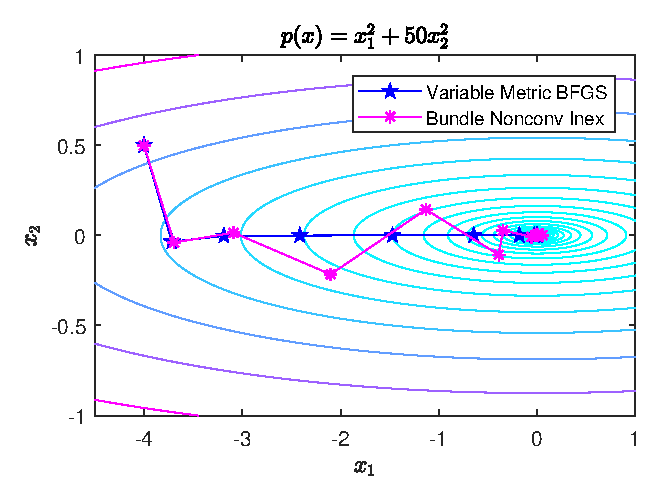
\includegraphics[width=\textwidth]{Pictures/Plots/final_parab.eps}
		\subcaption{Parabola, \(kappa = 2\), sequwnces of \(x_{hats}\); Noll:\(10|1\), Hare: \(28|12\)}
\end{subfigure}
\begin{subfigure}[t]{0.49\textwidth}
	\begin{center}
		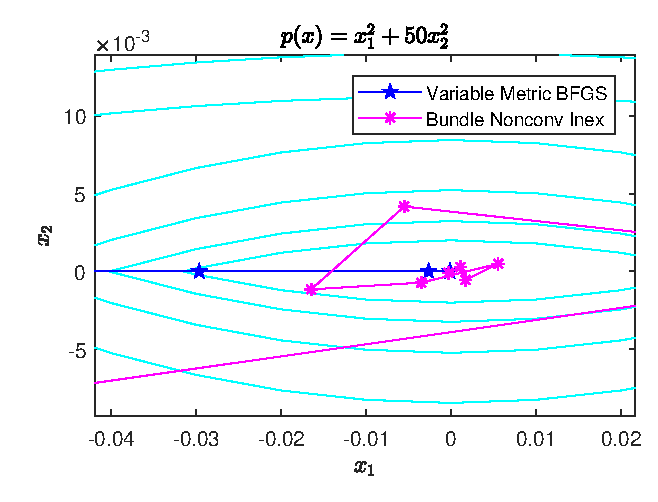
\includegraphics[width=\textwidth]{Pictures/Plots/final_parab_detail.eps}
		\subcaption{detail, many steps of Hare in the end}
	\end{center}
\end{subfigure}
\caption{}
\label{Im_Parab}
\end{figure}

\begin{figure}[H]
\begin{subfigure}[t]{0.49\textwidth}
		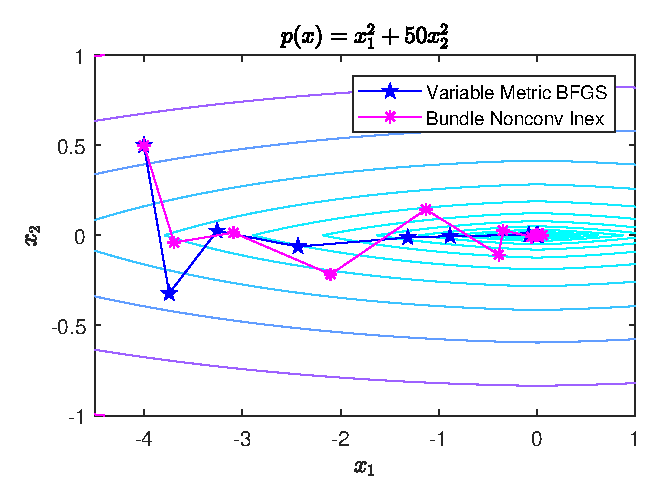
\includegraphics[width=\textwidth]{Pictures/Plots/final_nonsm_parab.eps}
		\subcaption{Parabola, \(kappa = 2\), sequwnces of \(x_{hats}\); Noll:\(21|9\), same for adapted, Hare: \(28|12\)}
\end{subfigure}
\begin{subfigure}[t]{0.49\textwidth}
	\begin{center}
		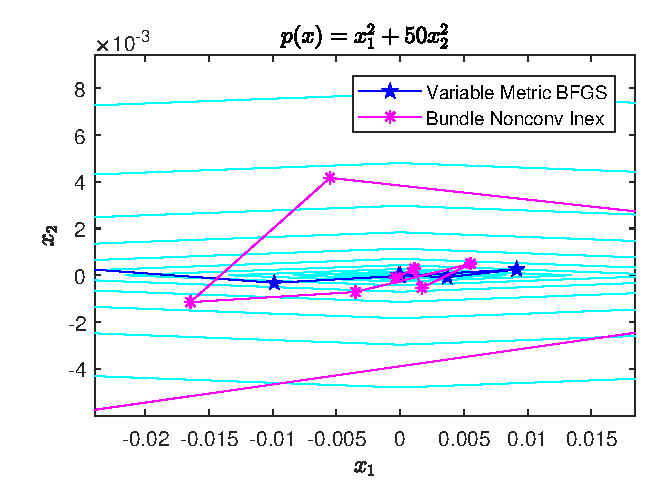
\includegraphics[width=\textwidth]{Pictures/Plots/final_nonsm_parab_detail.eps}
		\subcaption{detail}
	\end{center}
\end{subfigure}
\caption{}
\label{Im_Nonsm_Parab}
\end{figure}

\begin{figure}[H]
\begin{subfigure}[t]{0.49\textwidth}
		\includegraphics[width=\textwidth]{Pictures/Plots/steps_bar.eps}
		\subcaption{Parabola, \(kappa = 2\), sequwnces of \(x_{hats}\); Noll:\(21|9\), same for adapted, Hare: \(28|12\)}
\end{subfigure}
\begin{subfigure}[t]{0.49\textwidth}
	\begin{center}
		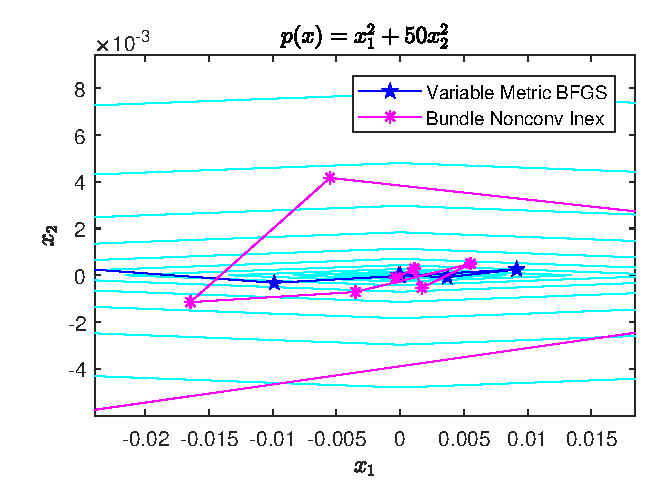
\includegraphics[width=\textwidth]{Pictures/Plots/final_nonsm_parab_detail.eps}
		\subcaption{detail}
	\end{center}
\end{subfigure}
\caption{}
\label{Im_Nonsm_Parab}
\end{figure}
\textcolor{red}{second example: nonsmooth version of the parabola
\[ p: \R^2 \to \R, \quad x \mapsto \Langle x, \frac{1}{2}Ax\Rangle + 0.5 |x_1|+25|x_2|\]
kink makes problem with second order information; different possibilities\\
\begin{enumerate}
	\item change nothing, just make sure \(Q\) bounded
	\item scale \(Q\) if it becomes too big \\
	advantage: not so much wrong information due to ``krummungs-Paradoxon''\\
	drawback: everxthing scaled -> direction wrong if kink only in one direction; have to decide when \(Q\) too big, because exiist functions with high curvature
	\item change only eigenvalue that got too high; check Change relative to last \(Q\) and stepsize
	\item bigger stepsizes?
\end{enumerate}
first and third variants make sense in example}



%\subsection{Subproblem Variable Metric}
%
%For comparision: Subproblem proximal bundle
%
%\begin{align}
	%&\min_{d \in \R^n, \xi \in \R} \xi + \frac{1}{2t_k}\|d\|^2 = \xi + \frac{1}{2}d^{\top}\left(\frac{1}{t_k}\mathbf{I}\right)d \\
	%&\text{s.t.} \quad f(\hat{x}^k)+{g^j}^{\top}d - e^k_j - \xi \leq 0, \quad j \in J_k
%\end{align}
%
%Subproblem variable metric:
%\begin{align}
	%&\min_{d \in \R^n, \xi in \R} \xi + \frac{1}{2}d^{\top}D_kd \\
	%&\text{s.t.} \quad f(\hat{x}^k)+{g^j}^{\top}d - e^k_j - \xi \leq 0, \quad j \in J_k
%\end{align}
%These are \(\R^{n+1}\) dimensional quadratic optimization problems.\\
%
%\textcolor{red}{Find out if \(D_k\) is diagonal matrix! Think not.} \\
%
%Approaches not so different. Instead of just scaling the identity \(\rightarrow\) induce ``curvature information'' via past subgradients. \\
%
%Dual proximal subproblem:
%\begin{align}
	%&\min_{\alpha \in \R^{|J_k|}} \frac{1}{2} \left(\sum_{j \in J_k}{\alpha_jg^j}\right)^{\top} t_k\mathbf{I} \left(\sum_{j \in J_k}{\alpha_jg^j}\right) + \sum_{j \in J_k}{\alpha_j e_j^k} \\
		%&\text{s.t.} \quad \sum_{j \in J_k}{\alpha_j} = 1 \text{ and } \alpha_j \geq 0 ~ j \in J_k
%\end{align}
%
%
%Dual variable metric subproblem:
%\begin{align}
	%&\min_{\alpha \in \R^{|J_k|}} \frac{1}{2} \left(\sum_{j \in J_k}{\alpha_jg^j}\right)^{\top} D^{-1}_k \left(\sum_{j \in J_k}{\alpha_jg^j}\right) + \sum_{j \in J_k}{\alpha_j e_j^k} \\
		%&\text{s.t.} \quad \sum_{j \in J_k}{\alpha_j} = 1 \text{ and } \alpha_j \geq 0 ~ j \in J_k
%\end{align}
%
%These are \(\R^{|J_k|}\) dimensional quadratic optimization problems. \\
%
%\textcolor{red}{check linear independent \(g^j\)'s.}

\begin{itemize}
	\item Hare Algo seems to be better in ``global'' optimization \\
	Noll seems to get stuck in local Minima more often
	\item different ``Versions'' of Noll: Q ``ignored'' near kinks because there no curvature, but seems be be ``infinite''
	\item the t-update Parameter has A LOT of influence on the performance of the algorithm
\end{itemize}